%\documentclass[11pt,a4paper]{article}
\documentclass[11pt
  , a4paper
  , article
  , oneside
%  , twoside
%  , draft
]{memoir}

\usepackage{control}
\usepackage[numbers]{natbib}
\usepackage{tabulary}
\usepackage{control}
\usepackage[numbers]{natbib}  
\definecolor{babypink}{rgb}{0.96, 0.76, 0.76}
\definecolor{blizzardblue}{rgb}{0.67, 0.9, 0.93}


\begin{document}
 
\newcommand{\technumber}{
  RAON Control-Document Series\\
  Revision : v0.1,   Release : January. 08. 2016}
\title{\textbf{Synology NAS GitLab Server 구축}}

\author{박미정\thanks{mijoy0909@ibs.re.kr} \\
  Rare Isotope Science Project\\
  Institute for Basic Science, Daejeon, South Korea
}
\date{\today}


\renewcommand{\maketitlehooka}{\begin{flushright}\textsf{\technumber}\end{flushright}}
%\renewcommand{\maketitlehookb}{\centering\textsf{\subtitle}}
%\renewcommand{\maketitlehookc}{C}
%\renewcommand{\maketitlehookd}{D}

\maketitle

\begin{abstract}
본 문서는 Synology NAS의 GitLab 패키지를 이용한 Git Server 구축 매뉴얼이다.
\end{abstract}


\chapter{GitLab 설치}
NAS가 제공하는 DSM의 패키지 센터에서 GitLab을 검색하여 설치한다.
GitLab 설치 시 아래 그림과 같이 종속패키지로 Docker, MariaDB도 함께 설치해야하며, 이들은 설치 볼륨 선택 후 설치를 진행한다.
\begin{figure}[h!]
	\centering
	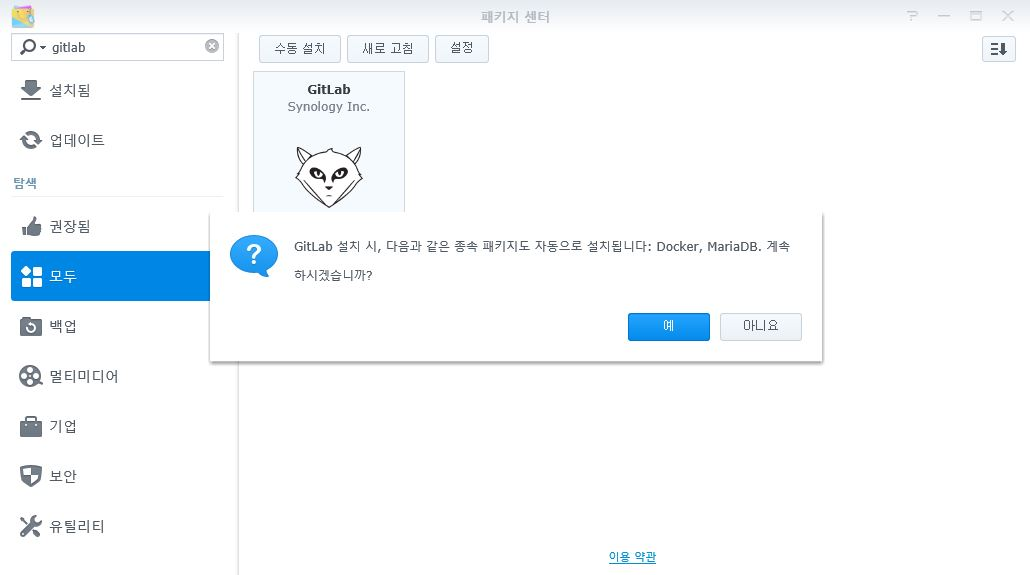
\includegraphics[width=0.65\textwidth]{./images/1.JPG} 
\end{figure}
\clearpage

GitLab은 설치 볼륨 선택 후 설치에 관한 사항을 아래와 같은 순서로 설정한다.
\begin{enumerate}
\item 데이터를 저장할 공유 폴더명과 GitLab의 HTTP, SSH 포트 번호를 설정한다.
\begin{figure}[h!]
	\centering
	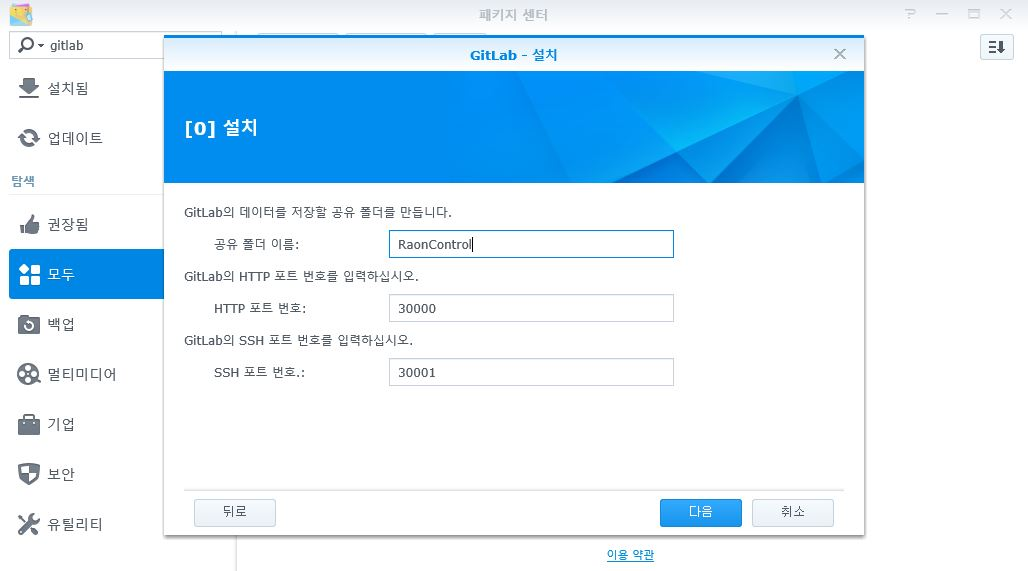
\includegraphics[width=0.99\textwidth]{./images/2.JPG}   
\end{figure}
\clearpage

\item 사용할 GitLab의 데이터베이스 이름을 입력한다. 
MariaDB의 Root패스워드는 따로 설정하지 않았다면 없다 (공백으로 둔다).\\ 
이는 MariaDB-MariaDB 패스워드 변경에서 변경 가능하다.
\begin{figure}[h!]
	\centering
	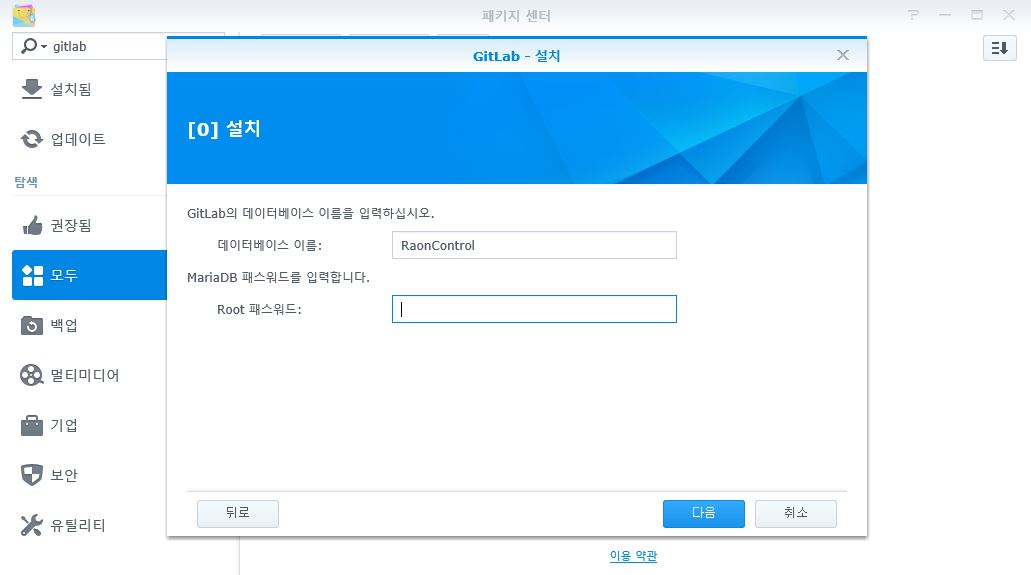
\includegraphics[width=0.99\textwidth]{./images/3.JPG}   
\end{figure}
\clearpage

\item GitLab이 사용할 도메인 이름과 관리자의 메일 계정을 입력한다.
\begin{figure}[h!]
	\centering
	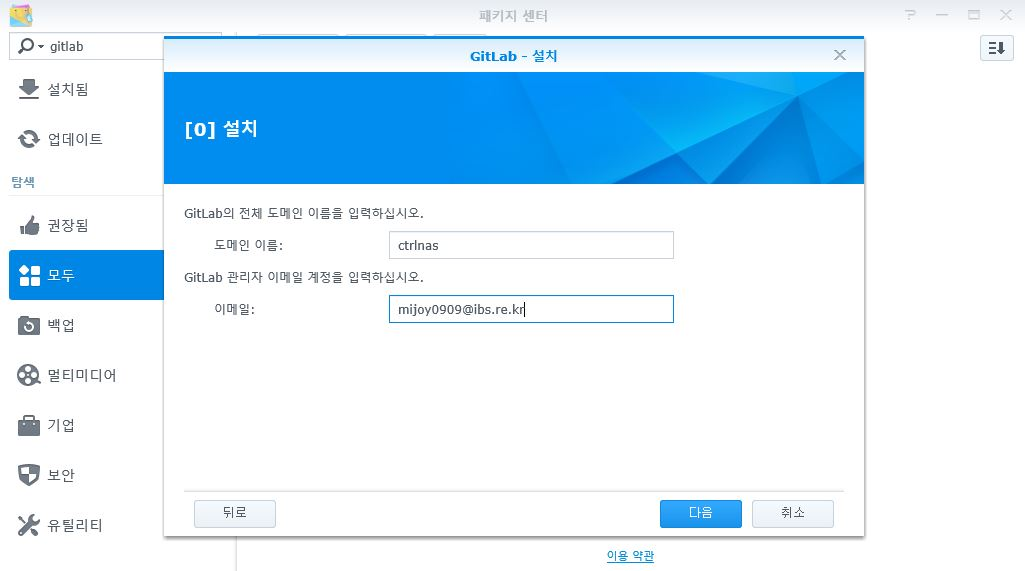
\includegraphics[width=0.99\textwidth]{./images/4.JPG} 
\end{figure}
\clearpage

\item SMTP는 사용 환경에 따라 설정한다. 우리는 메일 서버를 사용하지 않으므로 활성화하지 않았다.
\begin{figure}[h!]
	\centering
	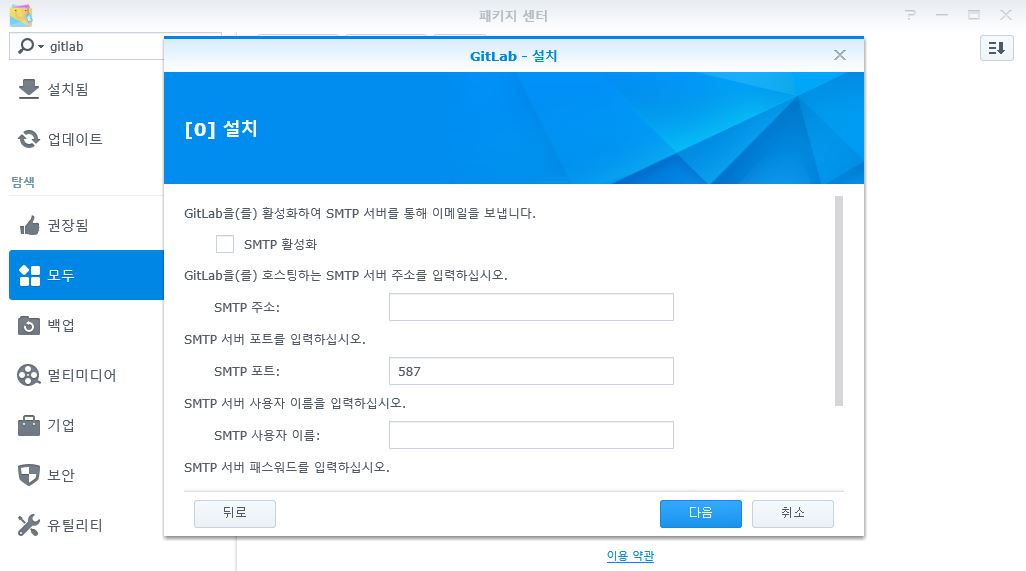
\includegraphics[width=0.99\textwidth]{./images/5.JPG}
	\caption{GitLab 설치 진행 화면 4}
\end{figure}
\clearpage

\item 설치 전 GitLab의 초기 Root 권한에 대한 정보를 알려준다. (root/5iveL!fe)
\begin{figure}[h!]
	\centering
	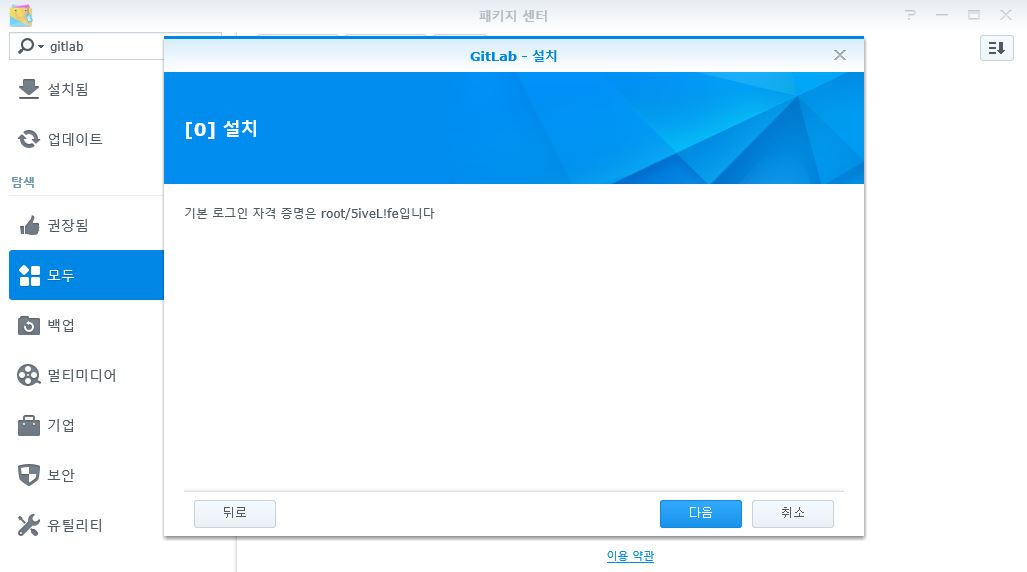
\includegraphics[width=0.99\textwidth]{./images/6.JPG}
\end{figure}
\clearpage

\item 모든 설정이 완료되었으므로, 설치를 수행한다.
\begin{figure}[h!]
	\centering
	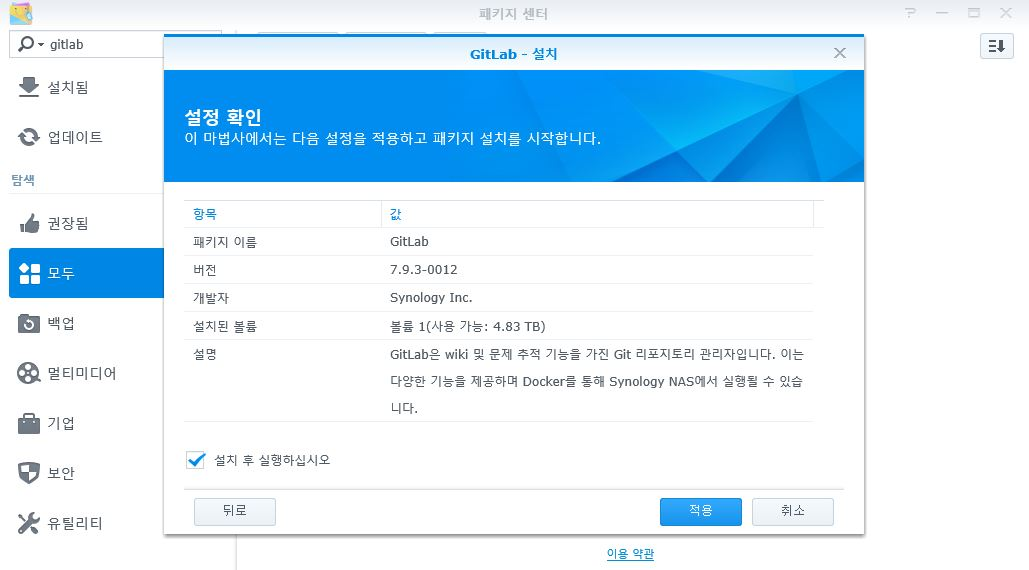
\includegraphics[width=0.99\textwidth]{./images/7.JPG}
\end{figure}

\begin{figure}[h!]
	\centering
	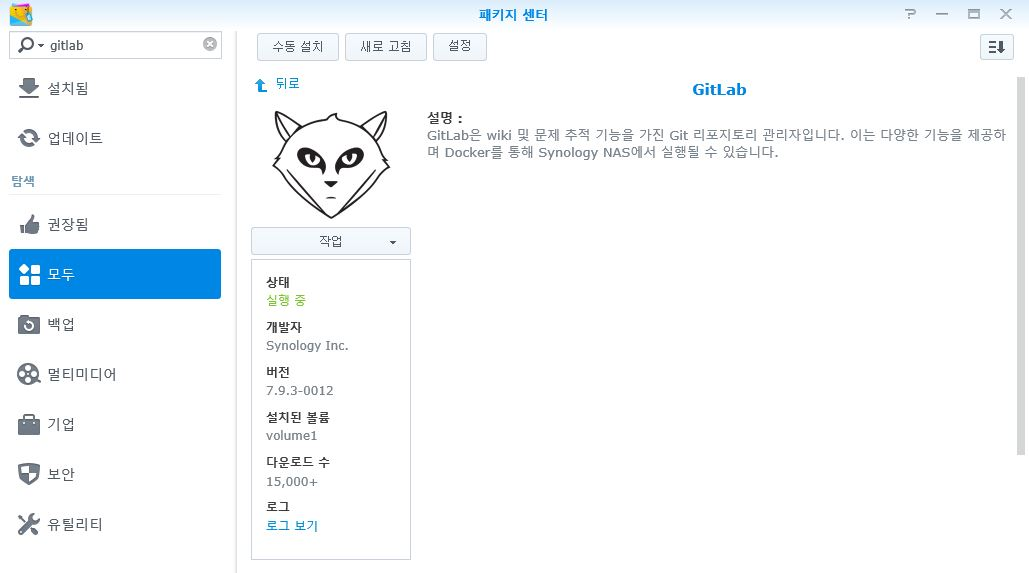
\includegraphics[width=0.99\textwidth]{./images/8.JPG}
\end{figure}
\end{enumerate}
\clearpage

\chapter{GitLab 설정}
\begin{itemize}
\item NAS 등록 정보
	\begin{itemize}
		\item[--] NAS : 10.1.5.5
		\item[--] NAS DMS : http://10.1.5.5:5000 
		\item[--] NAS GitLab : http://10.1.5.5:30000
	\end{itemize}
\end{itemize}

\begin{enumerate}
\item GibLab을 실행하면 아래와 같은 화면을 확인할 수 있다.이는 기존의 Github와 유사하다.
\begin{figure}[h!]
	\centering
	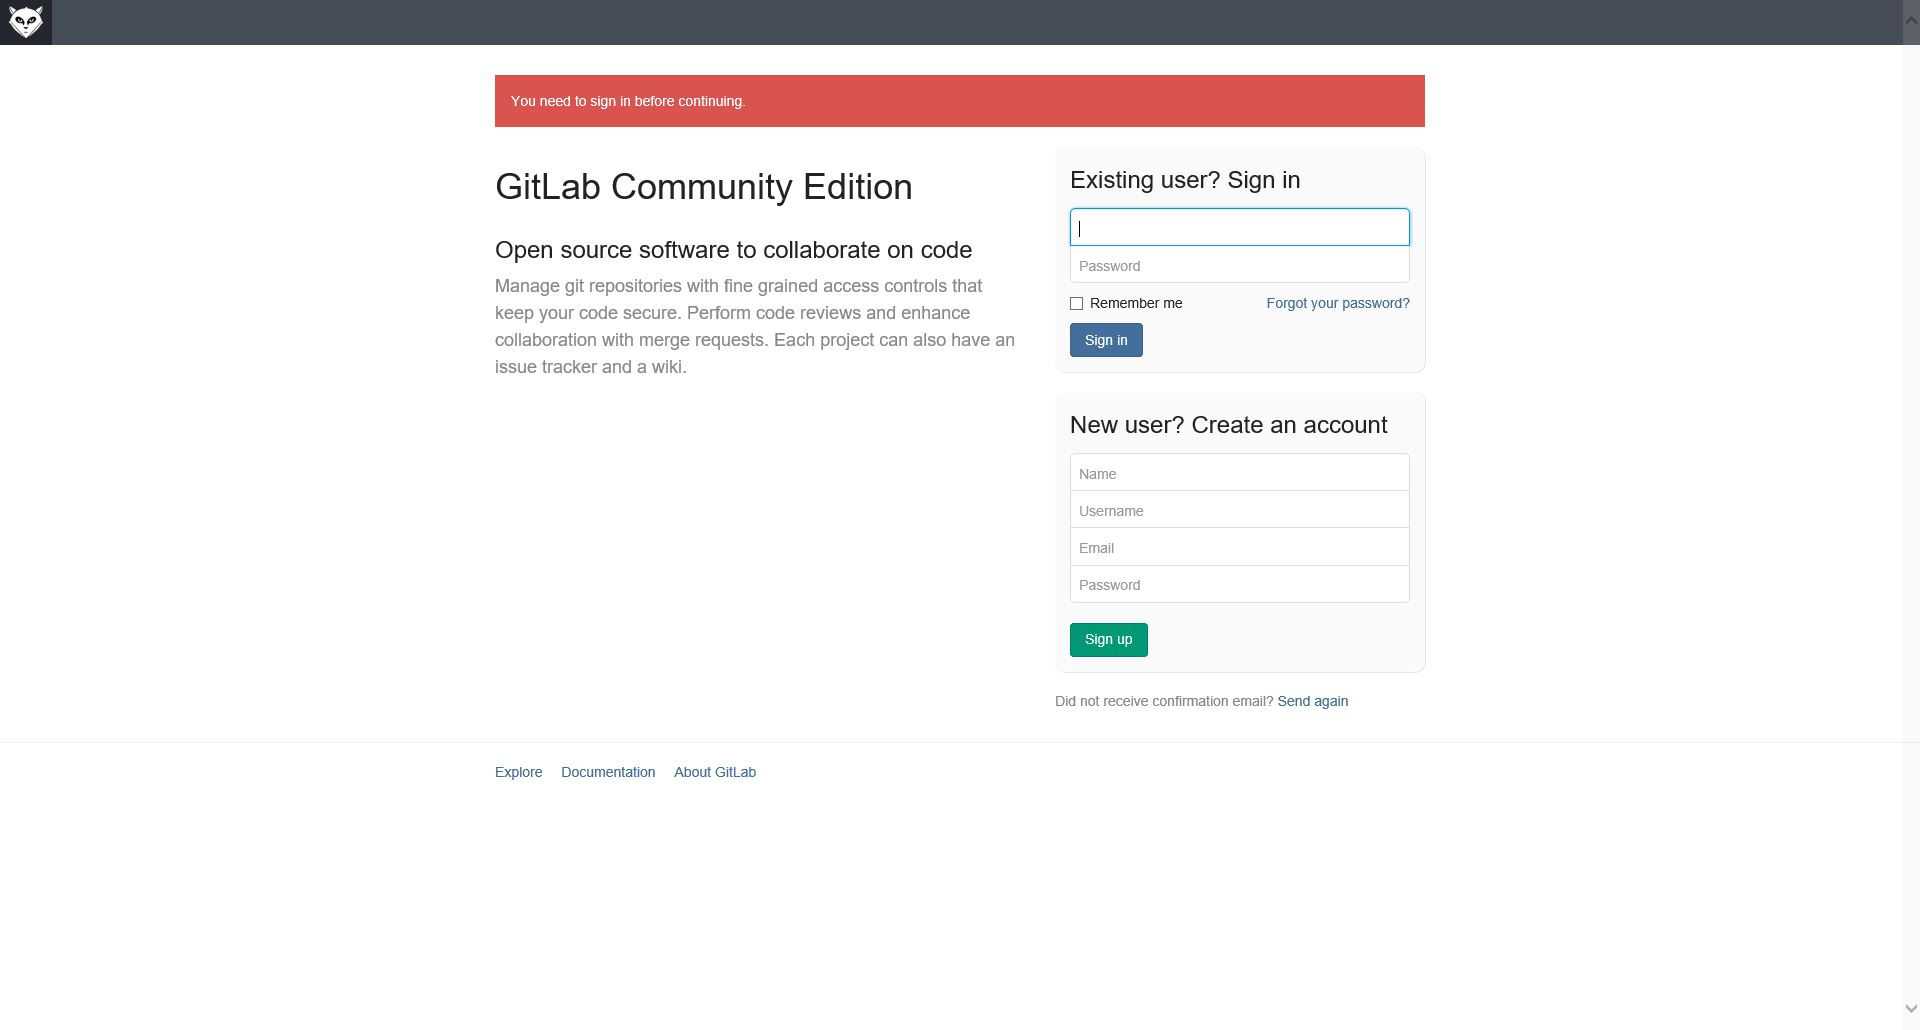
\includegraphics[width=0.99\textwidth]{./images/9.JPG}
\end{figure}

\item 앞서 알려준 초기 Root 권한으로 로그인하여, 패스워드를 변경한다.
\begin{figure}[h!]
	\centering
	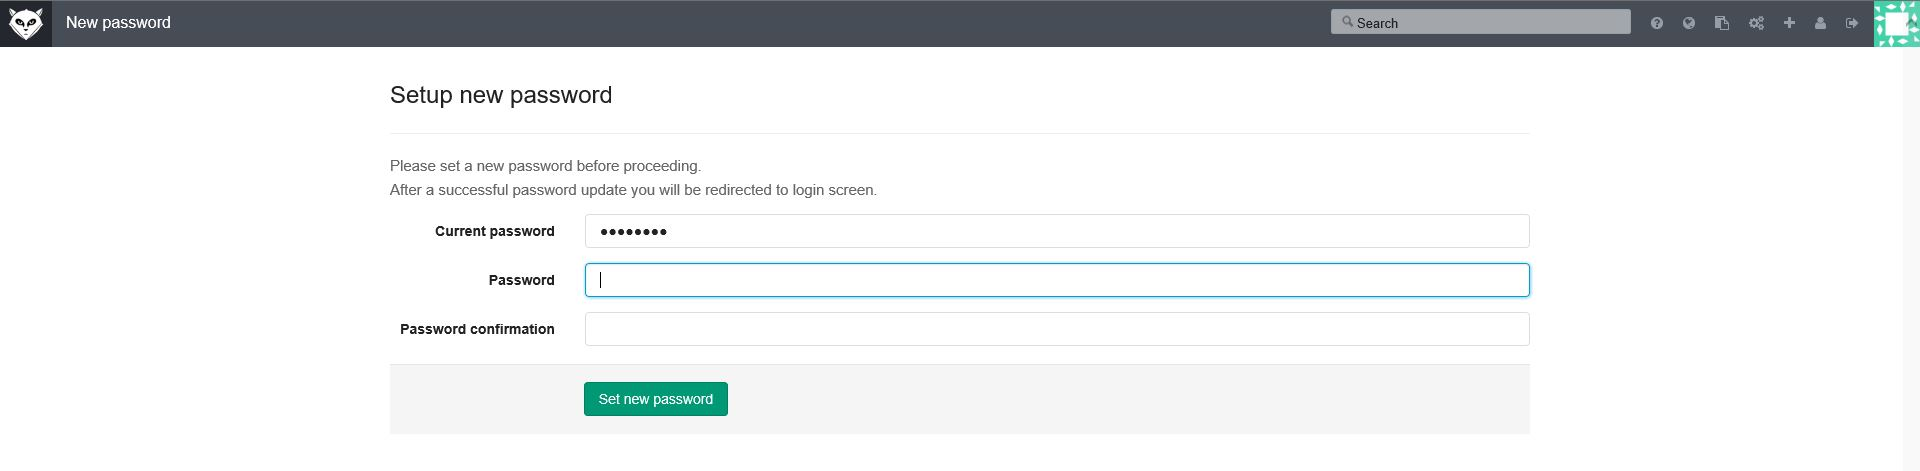
\includegraphics[width=0.99\textwidth]{./images/10.JPG}
\end{figure}
\clearpage

\item 새로운 그룹 및 프로젝트를 만든다. \\
제어그룹의 Git 프로젝트 그룹인 RaonControl을 생성하고, 기존의 git repository명을 프로젝트로 추가하였다.
\begin{figure}[h!]
	\centering
	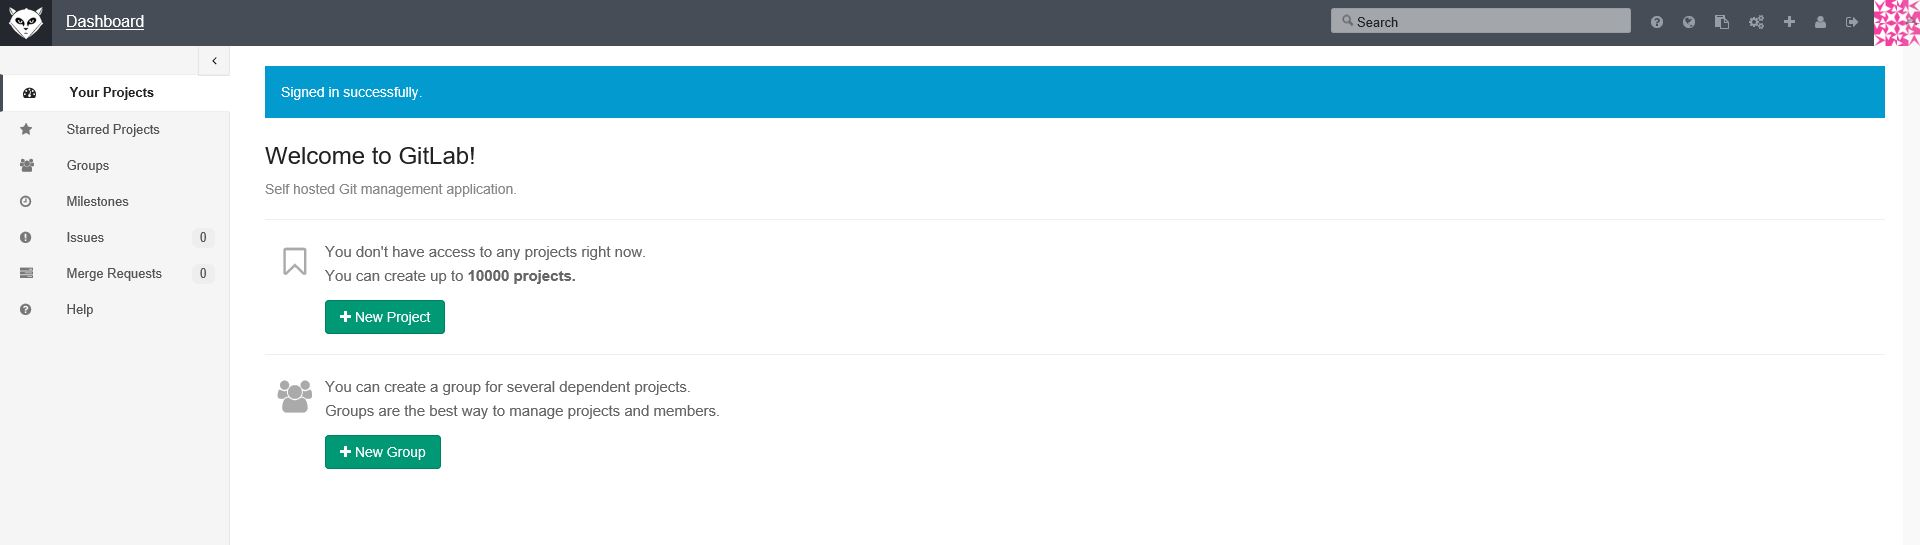
\includegraphics[width=0.99\textwidth]{./images/11.JPG}
\end{figure}
\begin{figure}[h!]
	\centering
	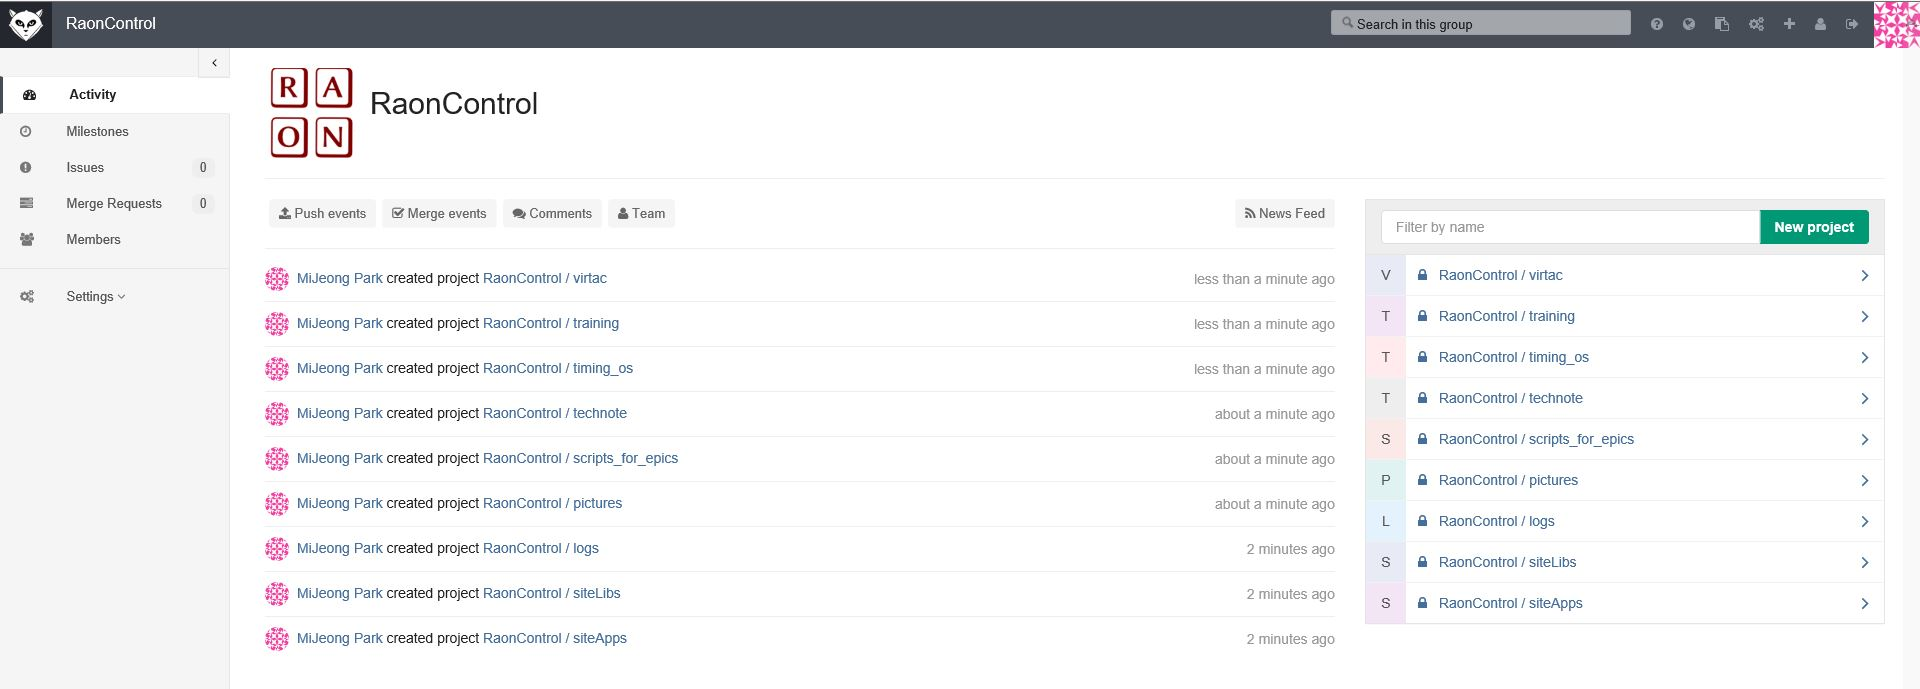
\includegraphics[width=0.99\textwidth]{./images/12.JPG}
\end{figure}
\end{enumerate}


\clearpage
\chapter{Git사용}
git의 사용 방법은 기존의 git 사용과 동일하다.

\begin{itemize}
\item[*] 기존 또는 새로운 리모트 저장소 등록
{\scriptsize
\begin{lstlisting}[style=termstyle, escapechar=!]
	mijoy0909@mjpark:~/git_RaonControl$ cd logs/
	mijoy0909@mjpark:~/git_RaonControl/logs$ git init
	Initialized empty Git repository in /home/mijoy0909/git_RaonControl/logs/.git/
	mijoy0909@mjpark:~/git_RaonControl/logs$ git add .
	mijoy0909@mjpark:~/git_RaonControl/logs$ git commit -m "first commit"
	[master (root-commit) 4a0e7d6] first commit
	50 files changed, 4181 insertions(+)
	(...)
	mijoy0909@mjpark:~/git_RaonControl/logs$ git remote add origin http://ctrlnas:30000/RaonControl/logs.git
	mijoy0909@mjpark:~/git_RaonControl/logs$ git push -u origin master 
	Username for 'http://ctrlnas:30000': mijoy
	Password for 'http://mijoy@ctrlnas:30000': 
	Counting objects: 55, done.
	Delta compression using up to 8 threads.
	Compressing objects: 100% (53/53), done.
	Writing objects: 100% (55/55), 838.50 KiB | 0 bytes/s, done.
	Total 55 (delta 4), reused 0 (delta 0)
	To http://ctrlnas:30000/RaonControl/logs.git
	* [new branch]      master -> master
	Branch master set up to track remote branch master from origin. 
\end{lstlisting}

}

\item[*] git clone
{\scriptsize
\begin{lstlisting}[style=termstyle, escapechar=!]
	mijoy0909@mjpark:~/git_RaonControl$ git clone http://ctrlnas:30000/RaonControl/logs.git
\end{lstlisting}
}
	
\item[*] git push
{\scriptsize
\begin{lstlisting}[style=termstyle, escapechar=!]
	mijoy0909@mjpark:~/git_RaonControl$ git push  
	mijoy0909@mjpark:~/git_RaonControl$ git push -u origin master 
\end{lstlisting}
}

\item[*] git  pull
{\scriptsize
\begin{lstlisting}[style=termstyle, escapechar=!]
	mijoy0909@mjpark:~/git_RaonControl$ git pull
\end{lstlisting}
}
\end{itemize}

\clearpage

\chapter{GitLab 사용 방법}
\begin{enumerate}
\item{사용자 계정 생성}
사용자 계정은 아래 그림과 같이 GitLab에서 생성하면 된다.
\begin{figure}[h!]
	\centering
	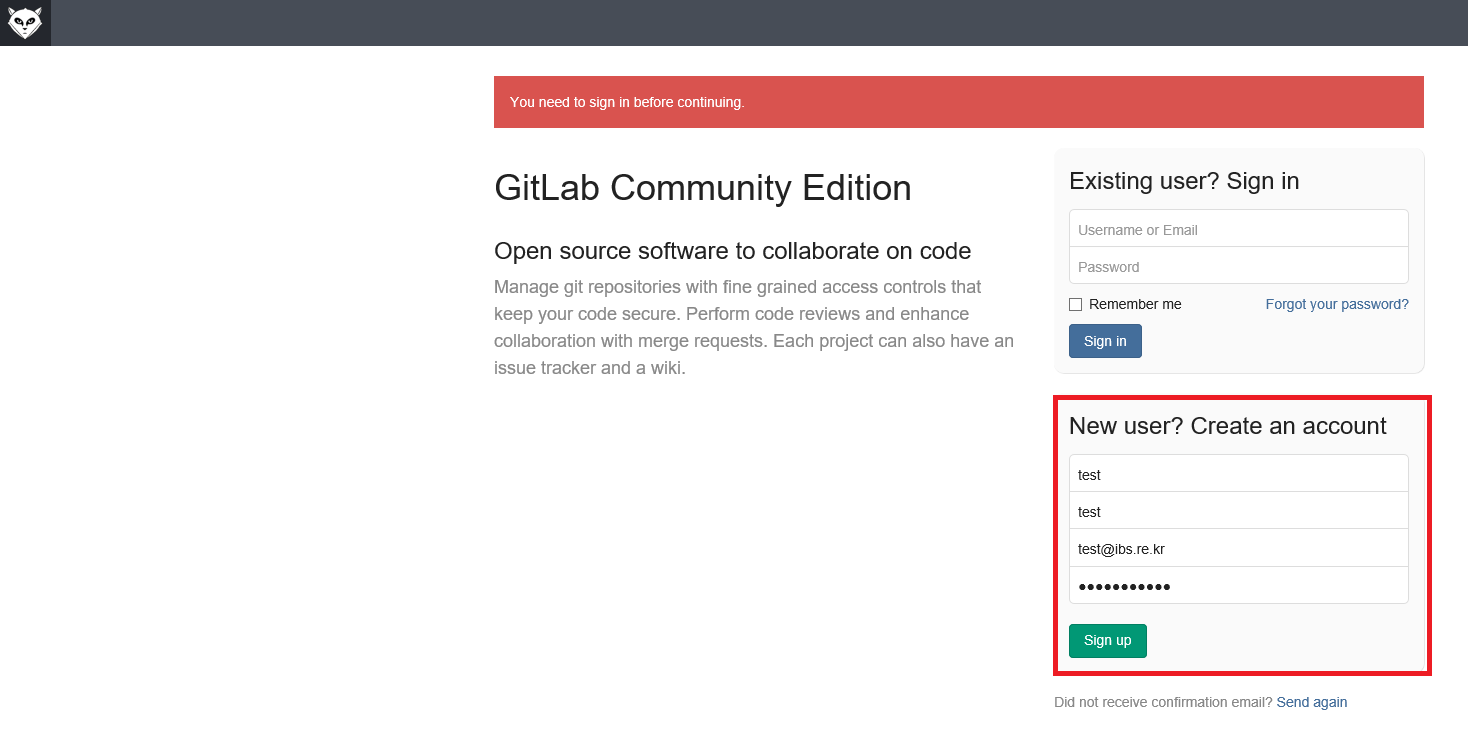
\includegraphics[width=0.99\textwidth]{./images/15.PNG}
\end{figure}

\item{사용자 계정 활성화}
원래 생성된 계정은 email 계정을 통해 확인을 하면 이용가능하지만, 이메일 서비스가 활성화 되지 않은 상황에서는 관리자 권한의 계정에서 계정 활성화가 가능하다.

- 관리자 권한으로 로그인 후 Admin area로 들어간다.
\begin{figure}[h!]
	\centering
	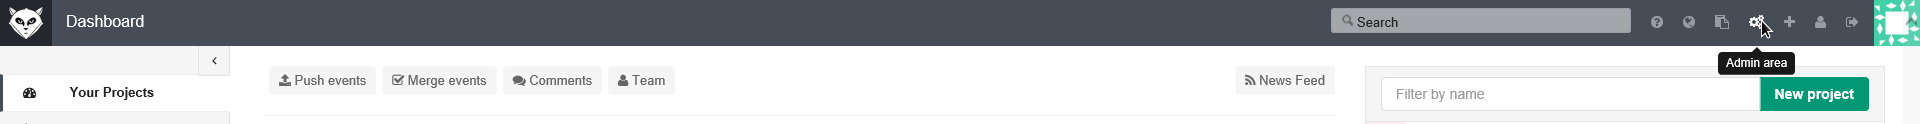
\includegraphics[width=0.99\textwidth]{./images/14.png}
\end{figure}

- Users의 숫자 클릭 후 권한을 부여하고자 하는 사용자 계정의 Edit버튼을 클릭한다.

\begin{figure}[h!]
	\centering
	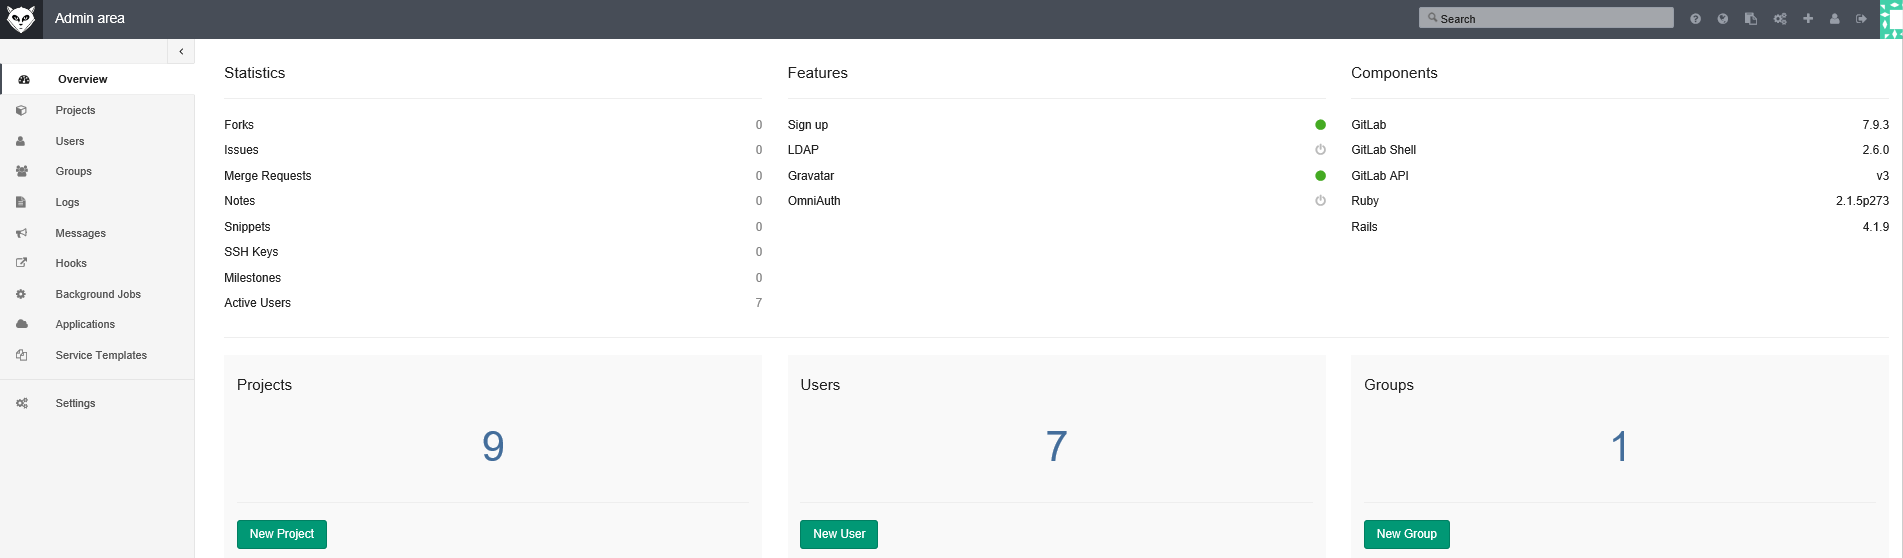
\includegraphics[width=0.99\textwidth]{./images/19.PNG}
\end{figure}
\begin{figure}[h!]
	\centering
	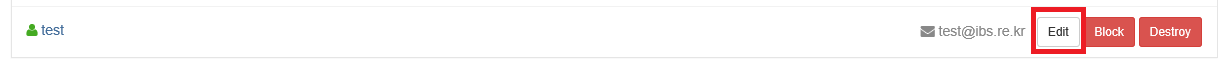
\includegraphics[width=0.99\textwidth]{./images/17.PNG}
\end{figure}

\vspace{2cm}
		
- 계정에 대한 설정 사항이 없다면, 그냥 Save changes 버튼을 클릭한다. (설정 사항이 있다면 변경한다.)
\begin{figure}[h!]
	\centering
	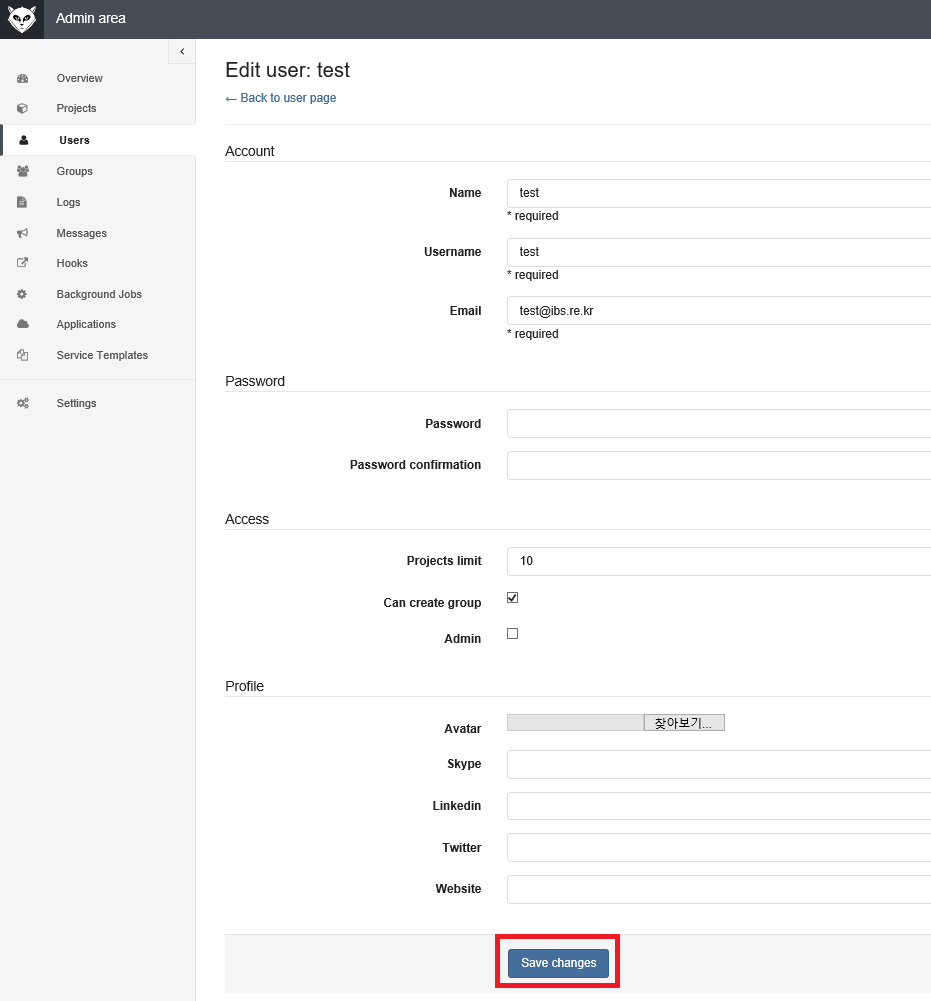
\includegraphics[width=0.99\textwidth]{./images/18.PNG}
\end{figure}

\clearpage

\item{사용자 Group에 추가}
Admin area에서 Groups를 누른 후 추가하고자 하는 사용자 검색 후 권한을 설정하고 추가한다.


\begin{figure}[h!]
	\centering
	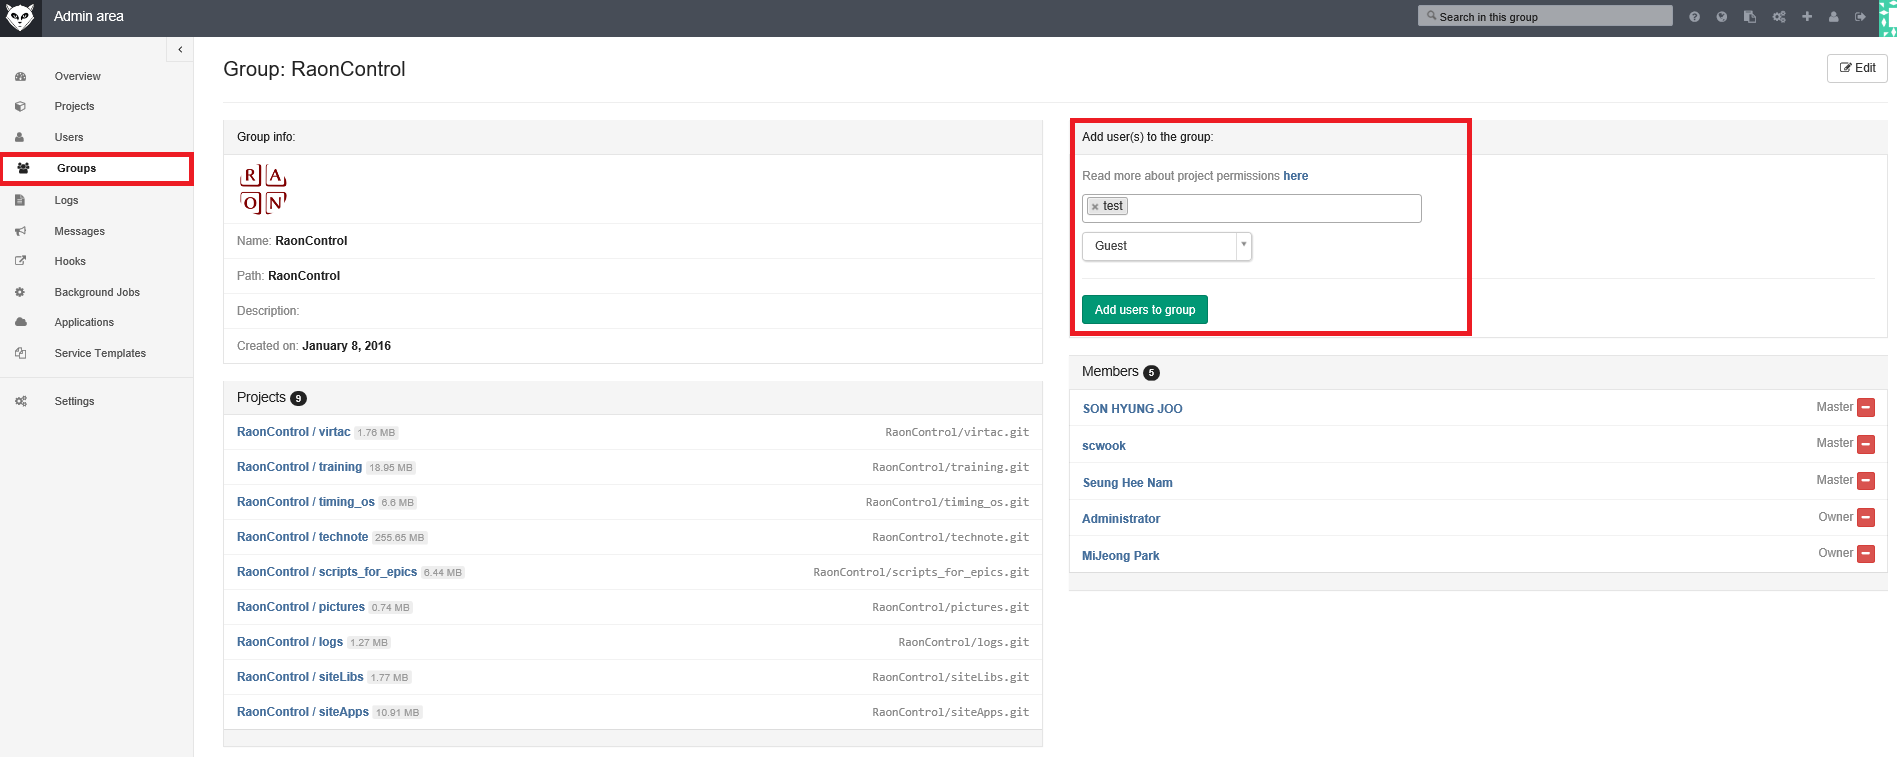
\includegraphics[width=0.99\textwidth]{./images/20.PNG}
\end{figure}

\item{사용자 프로젝트 권한 설정}
Group에 추가된 사용자는 그룹 내의 프로젝트에서 동일한 권한을 가진다. 따라서 게스트에게는 Group권한이 아닌 프로젝트 권한을 설정한다. 
- 게스트에게 권한을 주고자하는 프로젝트에서 상단의 Edit을 누른 후 왼쪽 사이드메뉴에서 Members를 선택한다.

\begin{figure}[h!]
	\centering
	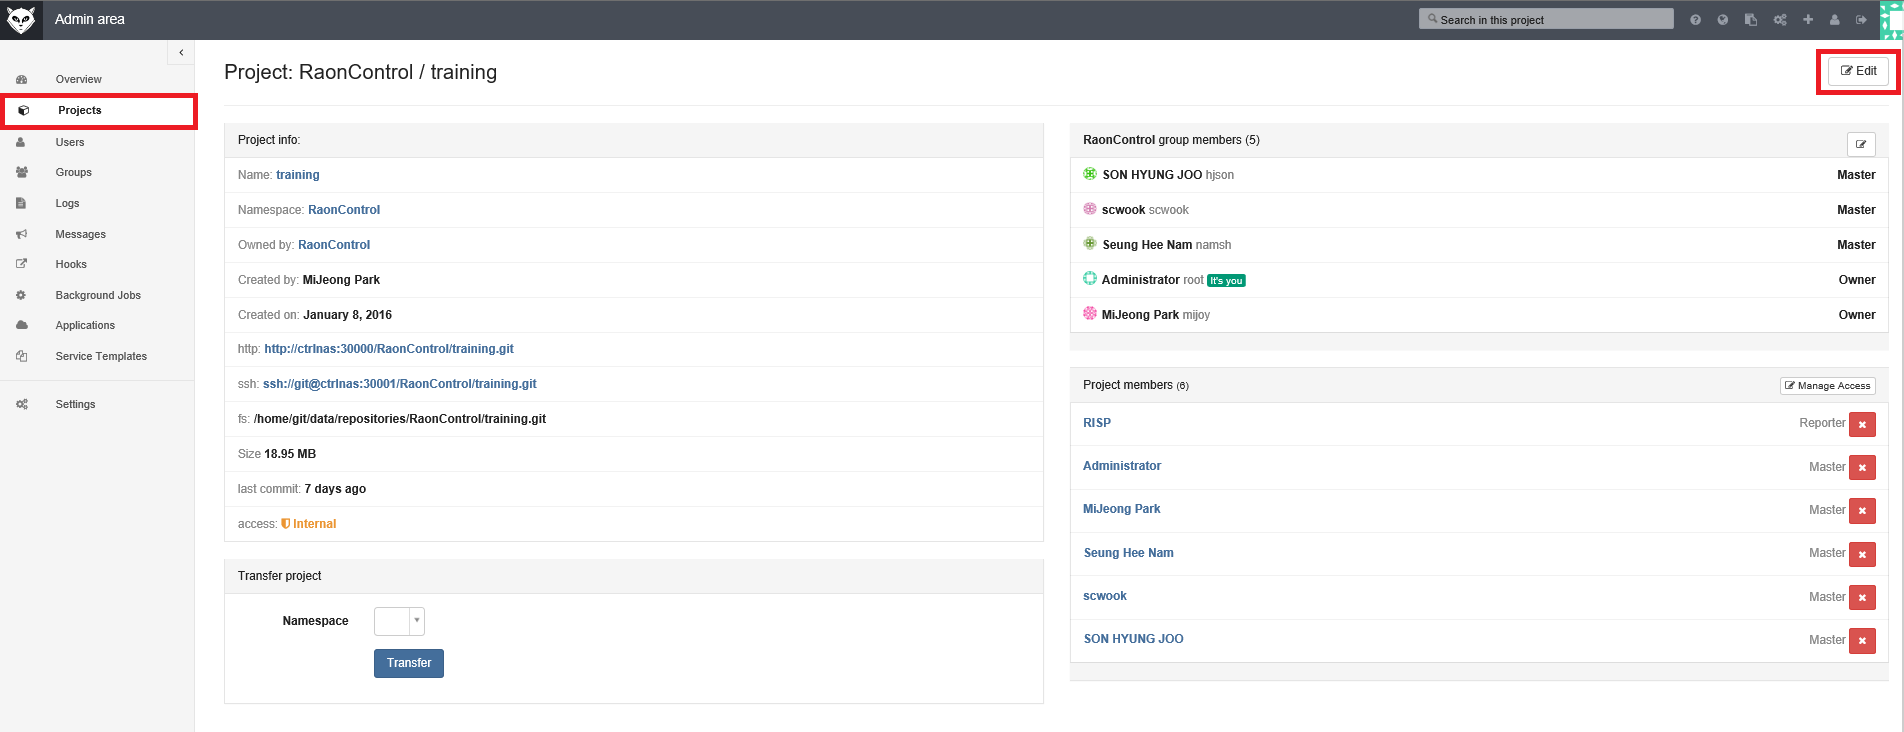
\includegraphics[width=0.99\textwidth]{./images/22.PNG}
\end{figure}

\clearpage

- Add members 버튼을 눌러 사용자를 추가한다.
\begin{figure}[h!]
	\centering
	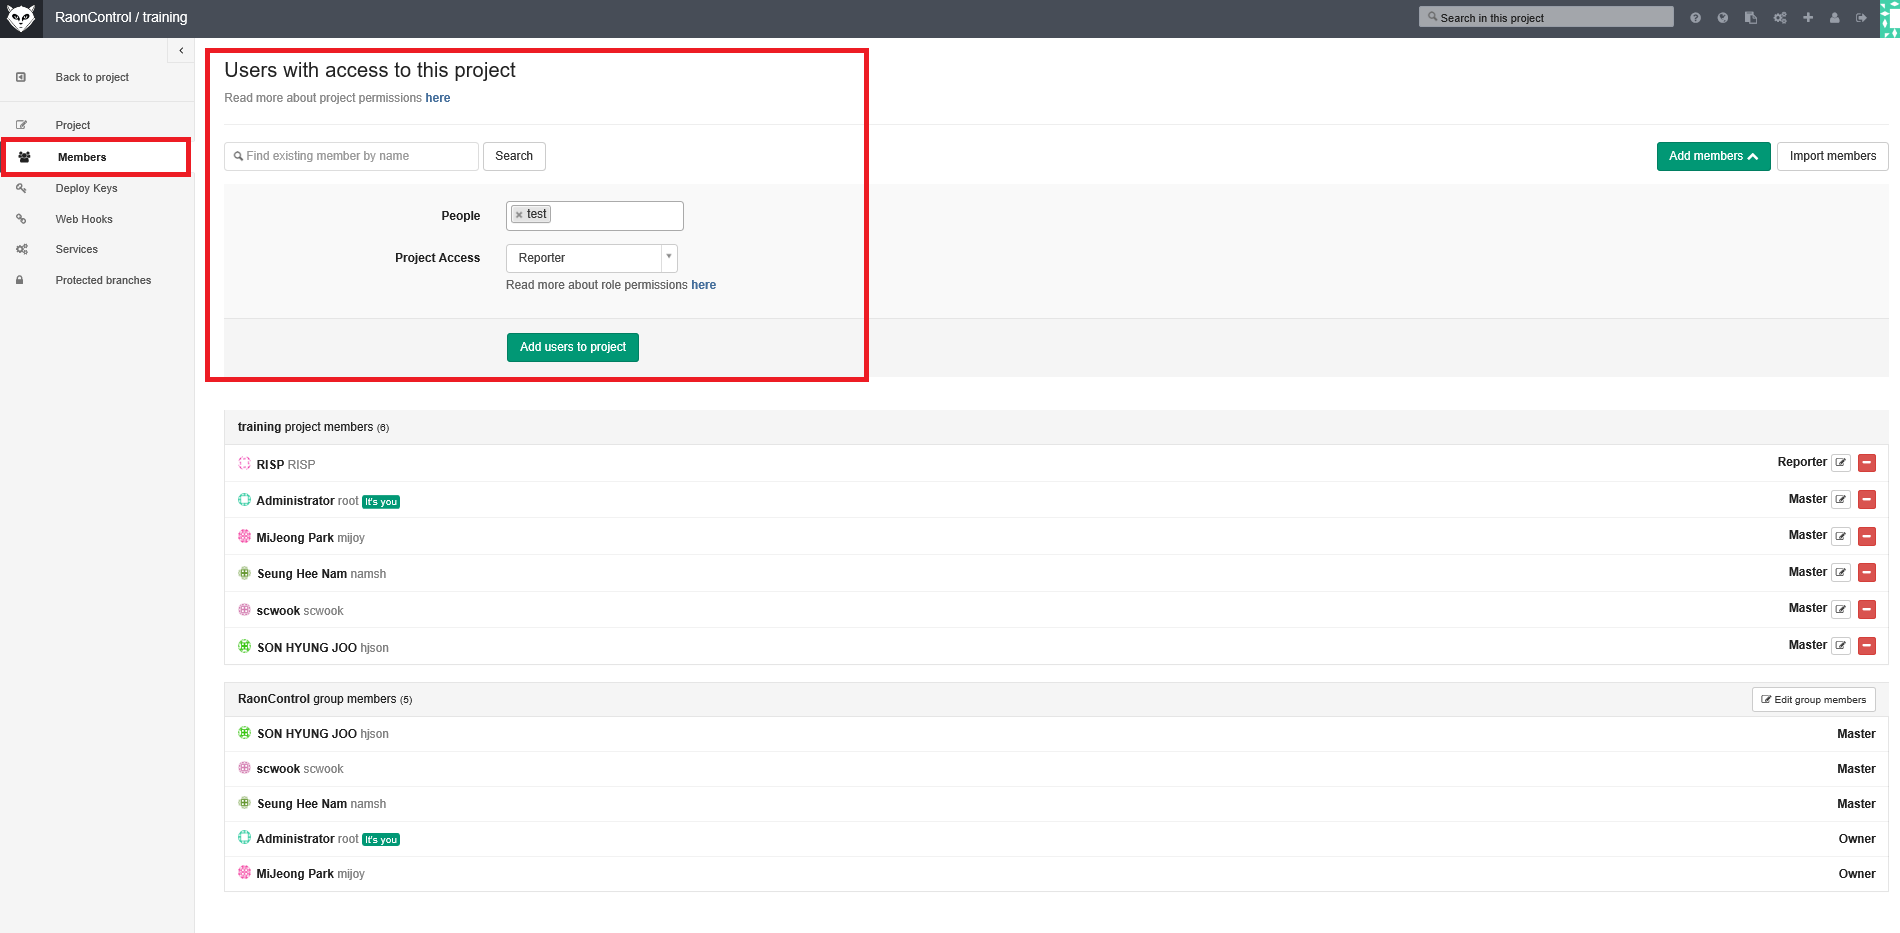
\includegraphics[width=0.99\textwidth]{./images/24.PNG}
\end{figure}

\end{enumerate}

- 게스트 계정 확인
게스트 계정에 접속하여 설정을 확인하면 아래와 같이 권한을 준 프로젝트에만 접속이 가능한 것을 확인할 수 있다.
\begin{figure}[h!]
	\centering
	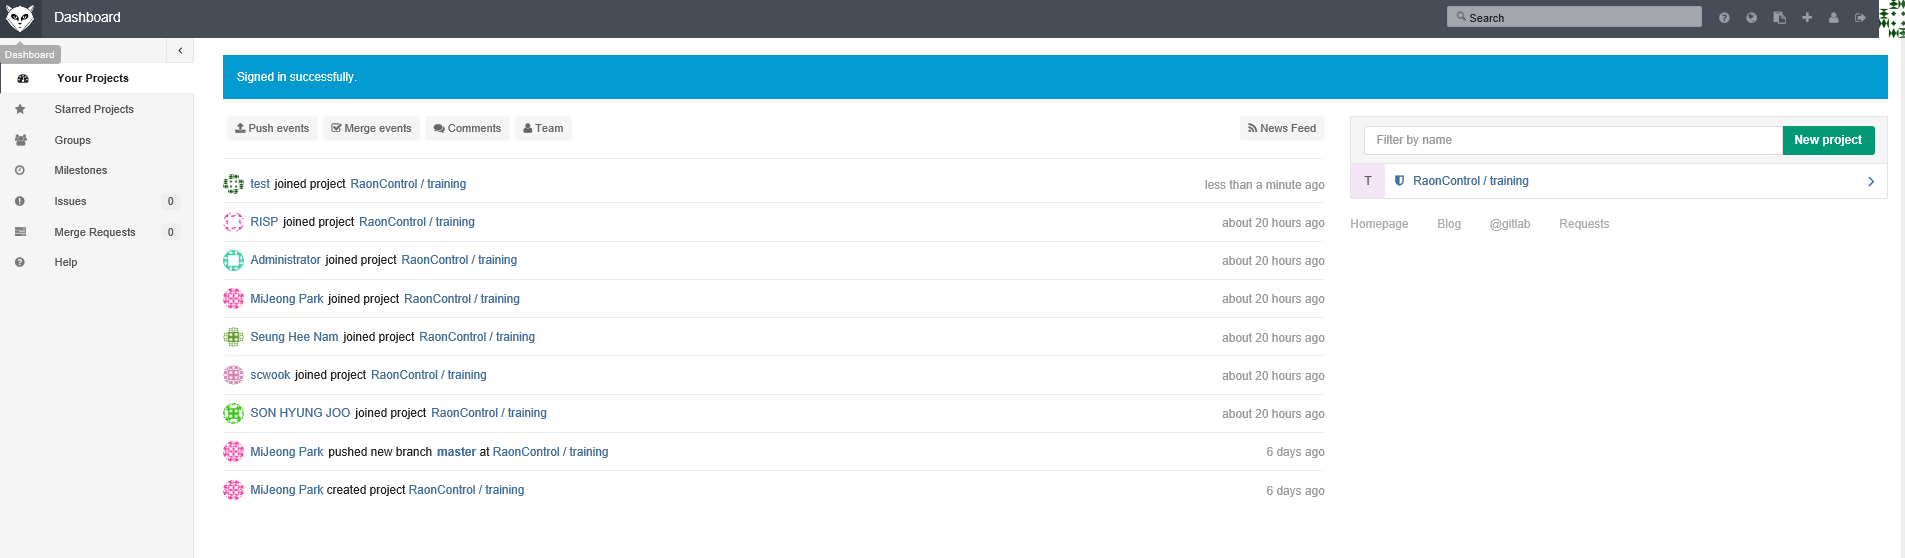
\includegraphics[width=0.99\textwidth]{./images/25.PNG}
\end{figure}

게스트 계정이 권한이 없는 프로젝트의 clone시에는 기존의 clone 메세지와 달리 아래와 같은 메세지를 확인할 수 있다.
{\scriptsize
	\begin{lstlisting}[style=termstyle, escapechar=!]
	mijoy0909@mjpark:~$ git clone http://ctrlnas:30000/RaonControl/training.git
	Cloning into 'training'...
	Username for 'http://ctrlnas:30000': test
	Password for 'http://test@ctrlnas:30000': 
	remote: Counting objects: 105, done.
	remote: Compressing objects: 100% (80/80), done.
	remote: Total 105 (delta 18), reused 105 (delta 18)
	Receiving objects: 100% (105/105), 18.84 MiB | 35.46 MiB/s, done.
	Resolving deltas: 100% (18/18), done.
	Checking connectivity... done.
	mijoy0909@mjpark:~$ 
	mijoy0909@mjpark:~$ git clone http://ctrlnas:30000/RaonControl/logs.git
	Cloning into 'logs'...
	Username for 'http://ctrlnas:30000': test
	Password for 'http://test@ctrlnas:30000': 
	!\colorbox{blizzardblue}{remote: Not Found}!
	!\colorbox{blizzardblue}{fatal: repository 'http://ctrlnas:30000/RaonControl/logs.git/' not found}!
	mijoy0909@mjpark:~$ 
	\end{lstlisting}
}

\clearpage

\chapter{Docker-GitLab push Error 해결}
기존 Github repository를 GitLab 서버로 push중 아래와 같은 문제점이 발생하였다.
\begin{itemize}
\item[*]ERROR1. [error: RPC failed; result=55, HTTP code = 0]	
{\scriptsize
\begin{lstlisting}[style=termstyle, escapechar=!]
	mijoy0909@mjpark:~/git_RaonControl/scripts_for_epics$ git push -u origin master 
	Counting objects: 160, done.
	Delta compression using up to 8 threads.
	Compressing objects: 100% (155/155), done.
	!\colorbox{babypink}{error: RPC failed; result=55, HTTP code = 0}!  12.42 MiB/s   
	fatal: The remote end hung up unexpectedly
	Writing objects: 100% (160/160), 52.84 MiB | 24.19 MiB/s, done.
	Total 160 (delta 7), reused 0 (delta 0)
	fatal: The remote end hung up unexpectedly
	Everything up-to-date
	mijoy0909@mjpark:~/git_RaonControl/scripts_for_epics$ 
\end{lstlisting}
}
\begin{itemize}
\item[-] 원인 : Git의 HTTP 버퍼 사이즈 문제
\item[-] 해결방법 : Git의 HTTP 버퍼 사이즈를 늘린다.
{\scriptsize
\begin{lstlisting}[style=termstyle, escapechar=!]
	mijoy0909@mjpark:~/git_RaonControl/scripts_for_epics$ git config http.postBuffer 524288000
\end{lstlisting}
}
\end{itemize}

\item[*]ERROR2. [error: RPC failed; result=22, HTTP code = 413]	
{\scriptsize
\begin{lstlisting}[style=termstyle, escapechar=!]
	mijoy0909@mjpark:~/git_RaonControl/technote$ git push -u origin master 
	Username for 'http://ctrlnas:30000': mijoy
	Password for 'http://mijoy@ctrlnas:30000': 
	Counting objects: 677, done.
	Delta compression using up to 8 threads.
	Compressing objects: 100% (674/674), done.
	Writing objects: 100% (677/677), 244.63 MiB | 23.75 MiB/s, done.
	Total 677 (delta 78), reused 0 (delta 0)
	!\colorbox{babypink}{error: RPC failed; result=22, HTTP code = 413}!
	fatal: The remote end hung up unexpectedly
	fatal: The remote end hung up unexpectedly
	Everything up-to-date
	mijoy0909@mjpark:~/git_RaonControl/technote$ 
\end{lstlisting}
}
	\begin{itemize}
	\item[-] 원인 : 웹서버에서 수신할 수 있는 최대 패킷 크기의 기본 값 보다 큰 사이즈의 파일이 push 될 경우 에러 발생 
	\item[-] 해결방법\citep{413error1}, \citep{413error2}, \citep{dockergitlab} : 
	
		\begin{enumerate}
		\item nginx.conf 파일 수정 (client\_max\_body\_size 옵션 추가)\\
		NGINX는 네트워크 확장성을 주목적으로 설계한 경량 HTTP 서버\citep{nginx}로 gitlab은 이를 사용한다. NGINX는 따로 설정을 하지 않으면 기본값인 1M로 데이터 업로드 용량을 제한한다. 따라서 업로드 용량 설정이 필요하다. 용량 설정의 최대값은 2G이다. 
		
		{\scriptsize
		\begin{lstlisting}[style=termstyle, escapechar=!]
		mijoy0909@mjpark:~$ ssh root@ctrlnas
		root@ctrlnas's password: 
		X11 forwarding request failed on channel 0
		
		BusyBox v1.16.1 (2015-11-12 18:01:52 CST) built-in shell (ash)
		Enter 'help' for a list of built-in commands.
		
		ctrlNAS> 
		ctrlNAS> vi /etc/nginx/nginx.conf 
		
		/*************************
		*       nginx.conf       *
		**************************/
		
		worker_processes    1;
		
		events {
		worker_connections  1024;
		}
		
		http {
			!\colorbox{blizzardblue}{client\_max\_body\_size 2G;}!
			include         mime.types;
			default_type    application/octet-stream;
		
			access_log      off;
			sendfile        on;
			send_timeout    300s;
			server_tokens   off;
			keepalive_timeout       65;
		
		server {
			listen      localhost:412;
			server_name _;
			location ~ \.php$ {
				fastcgi_index   index.php;
				fastcgi_pass    unix:/run/php-fpm/php-fpm.sock;
				fastcgi_param   SCRIPT_FILENAME $fastcgi_script_name;
				include         fastcgi_params;
			}
		
			location ~ /\.ht {
			deny all;
		
		
				}
			}
		}
				
		ctrlNAS> nginx -t             # Check the nginx error
		nginx: the configuration file /etc/nginx/nginx.conf syntax is ok
		nginx: configuration file /etc/nginx/nginx.conf test is successful
		ctrlNAS> nginx -s reload      # Restart nginx 
	\end{lstlisting}
	}
		
	\item php.ini 파일 수정 -> 파일 업로드 관련 설정 변경
	{\scriptsize
	\begin{lstlisting}[style=termstyle, escapechar=!]
	ctrlNAS> vi /etc/php/php.ini 

	/*************************
	*         php.ini        *
	**************************/
	
	[PHP]
	engine = On
	short_open_tag = On
	asp_tags = Off
	precision = 14
	output_buffering = 4096
	zlib.output_compression = Off
	implicit_flush = Off
	serialize_precision = 17
	disable_functions =
	disable_classes =
	zend.enable_gc = On
	expose_php = Off
	!\colorbox{blizzardblue}{max\_execution\_time = 24000}!     #default 240
	!\colorbox{blizzardblue}{max\_input\_time = 24000}!         #default60
	!\colorbox{blizzardblue}{memory\_limit = 12000M}!          #default128M
	error_reporting = E_ALL & ~E_NOTICE & ~E_STRICT & ~E_DEPRECATED
	display_startup_errors = Off
	log_errors = On
	log_errors_max_len = 1024
	ignore_repeated_errors = Off
	ignore_repeated_source = Off
	report_memleaks = On
	track_errors = Off
	html_errors = Off
	variables_order = "GPCS"
	request_order = "GP"
	register_argc_argv = Off
	auto_globals_jit = On
	!\colorbox{blizzardblue}{post\_max\_size = 24000M}!         #default32M
	default_mimetype = "text/html"
	default_charset = "UTF-8"
	include_path = "."
	extension_dir = "/usr/lib/php/modules"
	sys_temp_dir = "/var/services/tmp"
	enable_dl = Off
	file_uploads = On
	upload_tmp_dir = "/var/services/tmp"
	!\colorbox{blizzardblue}{upload\_max\_filesize = 12000M}!   #default32M
	max_file_uploads = 1000
	allow_url_fopen = On
	
	\end{lstlisting}
	}

	\item Docker-gitlab 관련 파일 수정
	\item[-] /volume1/@appstore/Docker-GitLab/config/synology\_gitlab
	{\scriptsize
	\begin{lstlisting}[style=termstyle, escapechar=!]
	/*************************
	*     synology_gitlab    *
	**************************/
	
	{"cpu_priority":0,"enable_publish_all_ports":false,"env_variables":[{"key":"GITLAB_HOST","value":"ctrlnas"},{"key":"GITLAB_PORT","value":"30000"},(...),!\colorbox{blizzardblue}{{"key":"NGINX\_MAX\_UPLOAD\_SIZE","value":"10000M"}}!,(...)]}
	\end{lstlisting}
	}
	
	
	\item[-] /usr/syno/etc/packages/Docker-GitLab/config 
	{\scriptsize
	\begin{lstlisting}[style=termstyle, escapechar=!]
	/*************************
	*         config         *
	**************************/
	
	(...)
	HOSTNAME="ctrlnas"
	ADMIN_EMAIL="mijoy0909@ibs.re.kr"
	!\colorbox{blizzardblue}{NGINX\_MAX\_UPLOAD\_SIZE="10000M"}!
	SMTP_ENABLE="false"
	(...)
	\end{lstlisting}
	}
		
	
	
	\item[-] /usr/syno/etc/packages/Docker/synology\_gitlab.config
	{\scriptsize
	\begin{lstlisting}[style=termstyle, escapechar=^]
	ctrlNAS> vi /usr/syno/etc/packages/Docker/synology_gitlab.config
	/*************************
	* synology_gitlab.config *
	**************************/
	
	{
	"cap_add" : [],
	(...)
	"env_variables" : [      
	{
	"key" : "GITLAB_HOST",
	"value" : "ctrlnas"
	},
	(...)
   
   ^\colorbox{blizzardblue}{\{}^                                                                     
	^\colorbox{blizzardblue}{"key" : "NGINX\_MAX\_UPLOAD\_SIZE",}^                                       
	^\colorbox{blizzardblue}{"value" : "10000M"}^                                                          
	^\colorbox{blizzardblue}{\},}^             
	], 
	(...)
	}
	
	ctrlNAS>
	ctrlNAS> reboot

	Broadcast message from root@ctrlNAS
	(/dev/pts/6) at 10:48 ...
	
	The system is going down for reboot NOW!
	
	ctrlNAS> Connection to ctrlnas closed by remote host.
	Connection to ctrlnas closed.
	mijoy0909@mjpark:~$  
	\end{lstlisting}
	}
	
	\item[+)] docker 재시작 방법
	{\scriptsize
	\begin{lstlisting}[style=termstyle]
	ctrlNAS> docker ps -a                   #check the gitlabapp container ID
	CONTAINER ID  IMAGE   COMMAND    CREATED   STATUS PORTS     NAMES
	74f1b2838932  sameersbn/gitlab:7.9.3  "/app/init app:start  2 hours ago  Up 32 minutes  443/tcp, 0.0.0.0:30001->22/tcp, 0.0.0.0:30000->80/tcp  synology_gitlab   
	686a5efa9909  redis:2.8.19            "/entrypoint.sh redi  2 hours ago  Up 32 minutes  6379/tcp                                               synology_gitlab_redis   
	
	ctrlNAS> docker restart 74f1b2838932    #docker restart container ID
	\end{lstlisting}
	}	
\end{enumerate}	
\end{itemize}	
\end{itemize}









\clearpage
\bibliographystyle{unsrtnat}
\bibliography{./refs}
\end{document}
